\documentclass[10pt]{report}
\usepackage[utf8]{inputenc}
\usepackage{amsfonts}
\usepackage{amsmath}
\usepackage{amssymb}
\usepackage{commath}
\usepackage[ngerman]{babel}
\usepackage{enumitem}
\usepackage{booktabs}
\usepackage{longtable}
\usepackage{relsize}
\usepackage{pgfplots}
\usepackage{csvsimple}
\usepackage{pgfplotstable}
\usepackage{siunitx}
\usepackage{fancyhdr}
\usepackage{color}
\usepackage{float}
\usepackage{listings}

\definecolor{mygreen}{RGB}{28,172,0} % color values Red, Green, Blue
\definecolor{mylilas}{RGB}{170,55,241}


\lstset{language=Matlab,%
    %basicstyle=\color{red},
    breaklines=true,%
    morekeywords={matlab2tikz},
    keywordstyle=\color{blue},%
    morekeywords=[2]{1}, keywordstyle=[2]{\color{black}},
    identifierstyle=\color{black},%
    stringstyle=\color{mylilas},
    commentstyle=\color{mygreen},%
    showstringspaces=false,%without this there will be a symbol in the places where there is a space
    %numbers=left,%
    %numberstyle={\tiny \color{black}},% size of the numbers
    %numbersep=9pt, % this defines how far the numbers are from the text
    emph=[1]{for,end,break},emphstyle=[1]\color{red}, %some words to emphasise
    %emph=[2]{word1,word2}, emphstyle=[2]{style},
}

\setlength\parindent{0pt}

\setcounter{chapter}{3}
\setcounter{secnumdepth}{3}
\setcounter{figure}{12}


\pagestyle{fancy}
\fancyhf{}
\lhead{GPET Versuch 4}
\rhead{Tim Luchterhand, Paul Nykiel}
\cfoot{\thepage}

\author{Tim Luchterhand, Paul Nykiel}
\title{GPET Versuch 4}

\begin{document}
        \maketitle
        \section{Ein- und Ausschaltvorgang einer Induktivität}
        \paragraph{Einführung}
        In diesem Versuch sollen die zeitlichen Verläufe des Stromes und der Spannung beim
        Schalten einer Induktivität untersucht werden. Verwenden Sie hierzu den in Abbildung
        ~\ref{fig:abb13} gezeigten Versuchsaufbau. Verwenden Sie einen Widerstand von $R=100\si{\ohm}$ und die
        Spule mit $n=250$ Windungen. Stellen Sie eine Rechteckspannung mit $f=10\si{k\hertz}$ ein.
        Bestimmen Sie den Verlauf der Spannung an der Spule, $U_2$, sowie des Stromes durch die
        Spule (über die Differenz der Spannungen $U_1$ und $U_2$) mit Hilfe des Oszilloskops und
        erklären Sie den charakteristischen Verlauf beider Größen.
        \begin{center}
            \begin{figure}[H]
                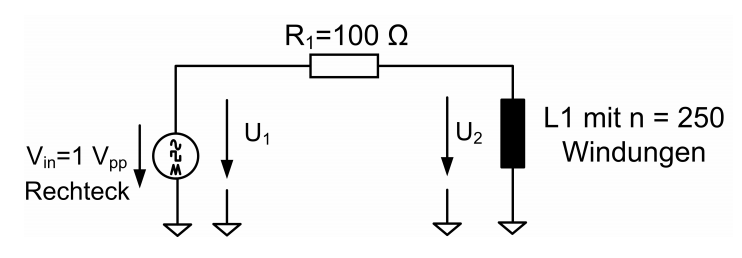
\includegraphics[width=\textwidth]{Abbildung13.png}
                \caption{Messaufbau um Strom- und Spannungsverlauf beim Schalten der Spannung
an einer Spule zu bestimmen}
                \label{fig  :abb13}
            \end{figure}
        \end{center}

        \subsection{Versuchsauswertung}

        \subsubsection{Screenshot}
        \paragraph{Aufgabe}
        Erstellen Sie einen Screenshot der Spannungs- und Stromverläufe.

        \paragraph{Protokoll}
        \begin{center}
            \begin{figure}[H]
                %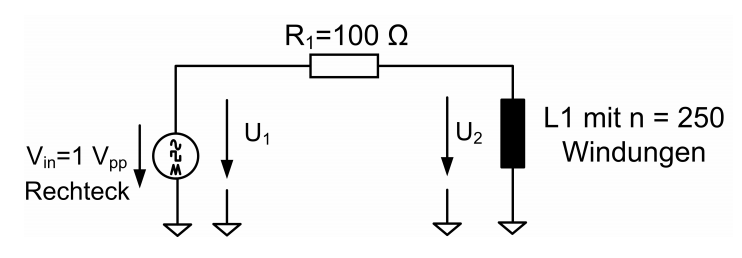
\includegraphics[width=\textwidth]{Abbildung13.png}
                \caption{Spannung an der Spule}
            \end{figure}
            \begin{figure}[H]
                %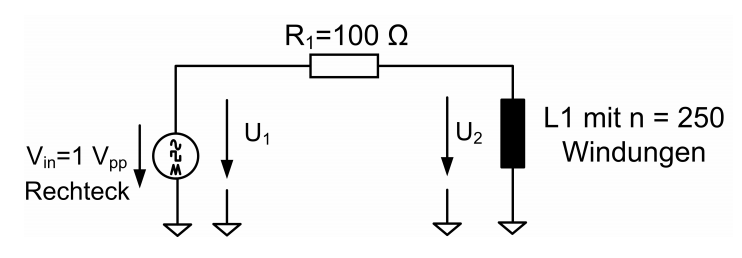
\includegraphics[width=\textwidth]{Abbildung13.png}
                \caption{Strom an der Spule}
            \end{figure}
        \end{center}

        \subsubsection{Erläuterung}
        \paragraph{Aufgabe}
        Erläutern Sie die Verläufe von Spannung und Strom.

        \paragraph{Protokoll}
        %TODO Text

        \section{Freie Schwingungen}
        \paragraph{Einführung}
        In diesem Versuch werden die freien Schwingungen eines LC Schwingkreises genauer untersucht.

        \subsection{Parasitäre Kapazität}
        \paragraph{Aufgabe}
        Bauen Sie hierzu zunächst die in Abbildung~\ref{fig:abb14} gezeigte Schaltung auf. Verwenden
        Sie die Spule mit $n = 1000$ Windungen.
        \begin{center}
            \begin{figure}[H]
                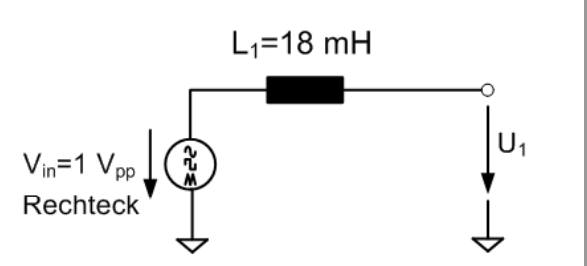
\includegraphics[width=\textwidth]{Abbildung14.png}
                \caption{Messaufbau zur Erzeugung einer freien Schwingung uber die Eigenresonanz einer Spule.}
                \label{fig:abb14}
            \end{figure}
        \end{center}

        \paragraph{Bemerkung}
        Die beobachtete Schwingung kommt durch die sogenannte Eigenresonanz der verwendeten
        Spule zu Stande. Die Spule weist neben ihrer Induktivität und ihrem
        Widerstand auch eine parasitäre Kapazität gemäß Abbildung 15 auf. Diese führt
        dazu, dass die Spule fur höhere Frequenzen nicht mehr als reine Induktivität wirkt
        sondern sich wie ein gedämpfter parallel-LC-Schwingkreis verhält.

        \begin{center}
            \begin{figure}[H]
                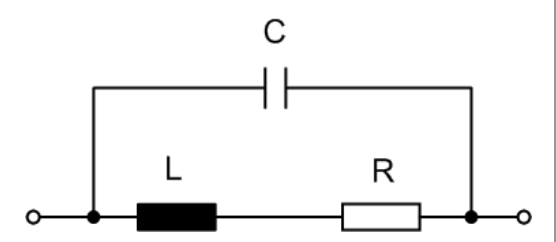
\includegraphics[width=\textwidth]{Abbildung15.png}
                \caption{Ersatzschaltbild einer realen Spule mit parasitärem Widerstand und parasitärer Kapazität.}
                \label{fig:abb15}
            \end{figure}
        \end{center}

        \paragraph{Aufgabe}
        Nehmen Sie den Verlauf der Spannung $U_1$ mit dem Oszilloskop auf und verwenden
        Sie die Cursorfunktion des Oszilloskops, um die Frequenz der Schwingung sowie die
        Abnahme der Amplitude der Schwingung zu messen.

        \subsubsection{Screenshot}
        \paragraph{Aufgabe}
        Erstellen Sie fur Ihre Versuchsauswertung einen Screenshot der Messung.

        \paragraph{Protokoll}
        \begin{center}
            \begin{figure}[H]
                %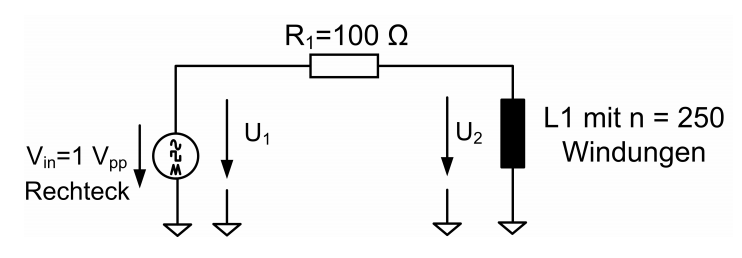
\includegraphics[width=\textwidth]{Abbildung13.png}
                \caption{Spannung an der Spule}
            \end{figure}
        \end{center}

        \subsubsection{Abschätzung der Kapazität}
        \paragraph{Aufgabe}
        Schätzen Sie mit Hilfe Ihrer Messung den Wert der parasitären Kapazität der
        verwendeten Spule ab.

        \paragraph{Protokoll}
        %TODO Formel überlegen


        \subsection{Schwingung am Kondensator}
        Bauen Sie als nächstes die in Abbildung~\ref{fig:abb16} dargestellte Schaltung auf. Verwenden
        Sie erneut die Spule mit $n = 1000$ Windungen und den Kondensator mit $C_1 =
        100 \si{\farad}$.

        \begin{center}
            \begin{figure}[H]
                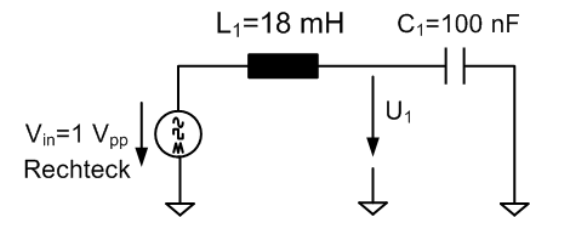
\includegraphics[width=\textwidth]{Abbildung16.png}
                \caption{Messaufbau zur Erzeugung einer freien Schwingung in einem Serien LC-Schwingkreis.}
                \label{fig:abb16}
            \end{figure}
        \end{center}

        \paragraph{Aufgabe}
        Nehmen Sie den Verlauf der Spannung $U_1$ mit dem Oszilloskop auf und verwenden
        Sie die Cursorfunktion des Oszilloskops, um die Frequenz der Schwingung
        sowie die Abnahme der Amplitude der Schwingung zu messen.

        \vspace{0.5cm}

        Erstellen Sie für Ihre Versuchsauswertung einen Screenshot der Messung.

        \paragraph{Protokoll}
        \begin{center}
            \begin{figure}[H]
                %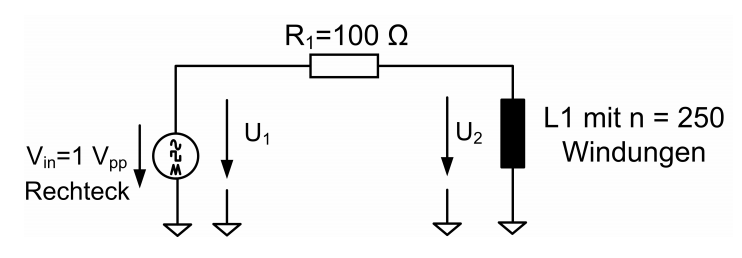
\includegraphics[width=\textwidth]{Abbildung13.png}
                \caption{Verlauf der Spannung am Kondensator}
            \end{figure}
        \end{center}

        \subsection{Veränderung der Schwingung}
        \paragraph{Aufbau}
        Bauen Sie nun die in Abbildung~\ref{fig:abb17} gezeigte Schaltung auf. Verwenden Sie erneut
        die Spule mit $n = 1000$ Windungen und den Kondensator mit $C_1 = 100\si{n\farad}$ sowie
        als Widerstand das Potentiometer.
        \begin{center}
            \begin{figure}[H]
                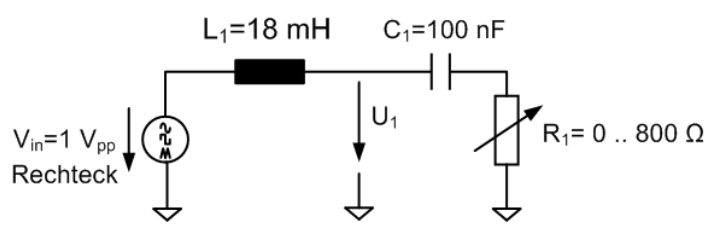
\includegraphics[width=\textwidth]{Abbildung17.png}
                \caption{Messaufbau Erzeugung einer freien Schwingung in einem Serien-LC Schwingkreis
                        mit erhöhter Dämpfung.}
                \label{fig:abb17}
            \end{figure}
        \end{center}

        \subsubsection{Spannungsverlauf}
        \paragraph{Aufgabe}
        Nehmen Sie den Verlauf der Spannung $U_1$ mit dem Oszilloskop auf. Stellen Sie
        mit dem Potentiometer nacheinander verschiedene Widerstandswerte zwischen
        $0$ und $800\si{\ohm}$ ein. Beobachten und beschreiben Sie die Änderungen im Verlauf
        der Schwingung.

        \paragraph{Protokoll}

        \subsubsection{Screenshot}
        \paragraph{Aufgabe}
        Nehmen Sie nun fur einen Wert von $R_1 \approx 15\si{\ohm}$ den Verlauf der Spannung $U_1$
        mit dem Oszilloskop auf und verwenden Sie die Cursorfunktion des Oszilloskops,
        um die Frequenz der Schwingung sowie die Abnahme der Amplitude
        der Schwingung zu messen. Erstellen Sie für Ihre Versuchsauswertung einen
        Screenshot dieser Messung.

        \paragraph{Protokoll}
        \begin{center}
            \begin{figure}[H]
                %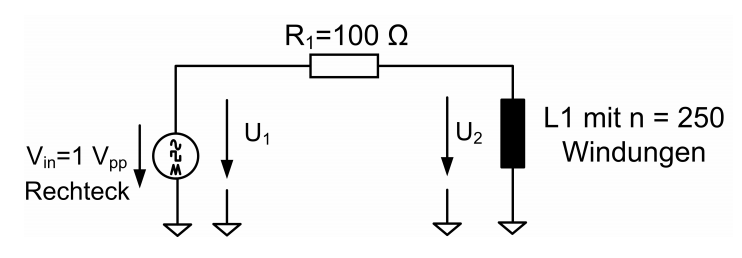
\includegraphics[width=\textwidth]{Abbildung13.png}
                \caption{Verlauf der Spannung am Kondensator}
            \end{figure}
        \end{center}

        \section{Spannungsüberhöhung}
        \paragraph{Aufgabe}
        In folgender Messung soll der Effekt der Spannungsüberhöhung in einem Serien-LC Schwingkreis
        untersucht werden. Errichten Sie hierzu die Schaltung nach Abbildung
        \ref{fig:abb18}. Verwenden Sie die Spule mit $n = 1000$ Windungen sowie einen Kondensator mit
        $C = 100\si{n\farad}$.

        \begin{center}
            \begin{figure}[H]
                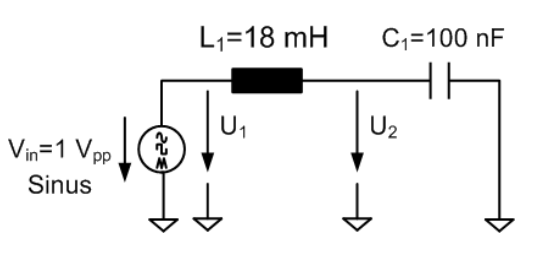
\includegraphics[width=\textwidth]{Abbildung18.png}
                \caption{Messaufbau zur Untersuchung der Spannungsüberhöhung in einem
                    Serien-LC-Schwingkreis.}
                \label{fig:abb18}
            \end{figure}
        \end{center}

        \subsection{Spannungsmaximum}
        \paragraph{Aufgabe}
        Bei welcher Frequenz erwarten Sie ein Maximum der Spannung $U_2$? Begrunden Sie
        Ihre Antwort.

        \paragraph{Protokoll}
        %TODO Text

        \subsection{Frequenzsweep}
        \paragraph{Aufgabe}
        Führen Sie mit Hilfe der MATLAB GUI einen Sweep der Eingangsfrequenz durch.
        Verwenden Sie dafür folgende Parameter: Type: Sweep frequency, peak-to-peak;
        Frequency sweep: logarithmic; Spannung 2 Vpp; Frequenz: 200 Hz bis 10 kHz; Anzahl
        der Punkte: 50. Fügen Sie eine Messkurve aus der GUI in Ihre Auswertung bei.
        Erzeugen Sie eine Grafik des durchgeführten Sweeps.

        \paragraph{Protokoll}


        \subsection{Übereinstimmung mit den theoretischen Werten}
        \paragraph{Aufgabe}
        Stimmt die Messung mit dem theoretischen Wert überein?

        \paragraph{Protokoll}
        %TODO Text


        \section{Induktionsschleife einer Ampelschaltung}
        Viele Ampelsysteme werden mittlerweile bedarfsgerecht geschaltet. Hierzu werden Sensoren
        benötigt, die ein Fahrzeug an einer Kreuzung erkennen können. Eine Fahrzeugerkennung
        wird üblicherweise über Induktionsschleifen im Boden vor einer Ampel realisiert. Mit
        modernen Induktionsschleifen kann nicht nur erkannt werden, ob ein Fahrzeug darüber
        steht, es kann sogar unterschieden werden, um welchen Fahrzeugtyp es sich handelt. So
        können beispielsweise LKW, PKW und Motorräder erkannt werden.
        Die Grundlagen solcher Sensoren wurden in den gerade eben durchgeführten Versuchen
        bereits behandelt. Wird Metall in die Nähe einer Spule gebracht, so ändert sich die
        Induktivität dieser Spule. Um diese Anderung einfach detektieren zu können, wird ein
        Schwingkreis verwendet.
        Bauen Sie die Ampelinduktionsschleife nach Abbildung \ref{fig:abb19} auf. Die Anordnung entspricht
        exakt derjenigen aus Versuch 3.3. Verwenden Sie eine Kapazität von $C = 100\si{n\farad}$ und die
        Spule mit $n = 1000$ Windungen. Aus Versuch 3.3 kennen Sie bereits die Resonanzfrequenz
        dieses LC-Schwingkreises.
        \begin{center}
            \begin{figure}[H]
                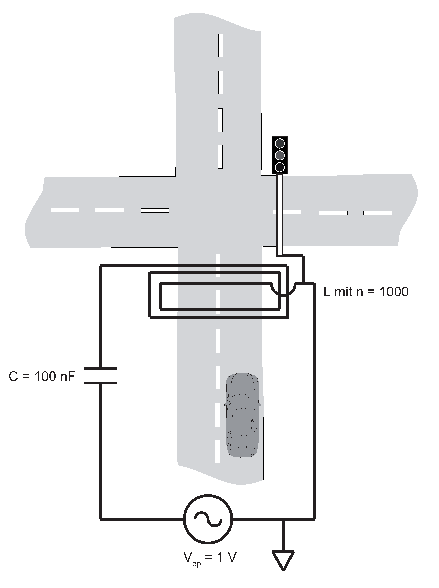
\includegraphics[width=\textwidth]{Abbildung19.png}
                \caption{Aufbau einer Induktionsschleife an einer Kreuzung.}
                \label{fig:abb19}
            \end{figure}
        \end{center}

        \subsection{Resonanzfrequenz}
        \paragraph{Aufgabe}
        Stellen Sie die Frequenz des Signalgenerators auf die eben ermittelte Resonanzfrequenz
        des LC-Schwingkreises ein und beobachten Sie die Spannung $U_2$ mit Hilfe des
        Oszilloskops. Setzen Sie Marker, um charakteristische Werte zu messen und nehmen
        Sie einen Screenshot auf.

        \paragraph{Protokoll}


        \subsection{Eisenkern}
        \paragraph{Aufgabe}
        Führen Sie nun einen Eisenkern in die Spule ein und beobachten Sie die Veränderung
        der Amplitude der Spannung $U_2$. Interpretieren Sie Ihre Beobachtung.

        \paragraph{Protokoll}


        \subsection{Frequenzsweep}
        \paragraph{Aufgabe}
        Wiederholen Sie nun den Frequenz-Sweep aus Versuch 3.3 mit Eisenkern in der
        Spule. Was stellen Sie fest? Interpretieren Sie Ihre Ergebnisse und erstellen Sie für
        Ihre Unterlagen eine Grafik des zweiten Frequenz Sweeps.

        \paragraph{Protokoll}


        \section{Analyse einer unbekannten Schaltung}
        In diesem Versuch soll das Verhalten einer unbekannten Schaltung, einer sogenannten
        Blackbox (BB) untersucht werden. Hierzu steht Ihnen im Rahmen dieses Versuchs eine
        mit BB1 beschriftete Blackbox zur Verfugung. Alle möglichen Schaltungskombinationen,
        die sich im Inneren der Blackbox befinden können, sind in Abbildung \ref{fig:abb21} dargestellt.
        Messen Sie die Transferfunktion der BB mit Hilfe des Schaltungsaufbaus in Abbildung
        \ref{fig:abb20}. Verwenden Sie hierzu einen Sweep mit einer unteren Frequenz von $1\si{\hertz}$, einer oberen
        Frequenz von $250\si{k\hertz}$ und einer Auflösung von $200$ Punkten.

        \begin{center}
            \begin{figure}[H]
                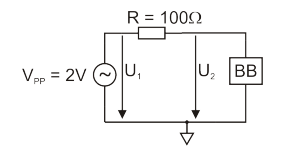
\includegraphics[width=\textwidth]{Abbildung20.png}
                \caption{Messaufbau zum Analysieren der BB}
                \label{fig:abb20}
            \end{figure}
            \begin{figure}[H]
                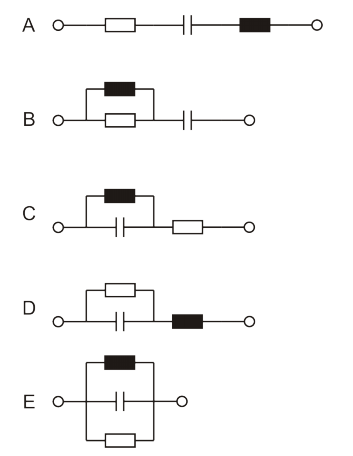
\includegraphics[width=\textwidth]{Abbildung21.png}
                \caption{Mögliche Schaltungen der BB}
                \label{fig:abb21}
            \end{figure}
        \end{center}


\end{document}
